\documentclass[journal]{vgtc}                % final (journal style)
%\documentclass[review,journal]{vgtc}         % review (journal style)
%\documentclass[widereview]{vgtc}             % wide-spaced review
%\documentclass[preprint,journal]{vgtc}       % preprint (journal style)

%% Uncomment one of the lines above depending on where your paper is
%% in the conference process. ``review'' and ``widereview'' are for review
%% submission, ``preprint'' is for pre-publication, and the final version
%% doesn't use a specific qualifier.

%% Please use one of the ``review'' options in combination with the
%% assigned online id (see below) ONLY if your paper uses a double blind
%% review process. Some conferences, like IEEE Vis and InfoVis, have NOT
%% in the past.

%% Please note that the use of figures other than the optional teaser is not permitted on the first page
%% of the journal version.  Figures should begin on the second page and be
%% in CMYK or Grey scale format, otherwise, colour shifting may occur
%% during the printing process.  Papers submitted with figures other than the optional teaser on the
%% first page will be refused. Also, the teaser figure should only have the
%% width of the abstract as the template enforces it.

%% These few lines make a distinction between latex and pdflatex calls and they
%% bring in essential packages for graphics and font handling.
%% Note that due to the \DeclareGraphicsExtensions{} call it is no longer necessary
%% to provide the the path and extension of a graphics file:
%% 
\includegraphics{diamondrule} is completely sufficient.
%%
\ifpdf%                                % if we use pdflatex
  \pdfoutput=1\relax                   % create PDFs from pdfLaTeX
  \pdfcompresslevel=9                  % PDF Compression
  \pdfoptionpdfminorversion=7          % create PDF 1.7
  \ExecuteOptions{pdftex}
  \usepackage{graphicx}                % allow us to embed graphics files
  \DeclareGraphicsExtensions{.pdf,.png,.jpg,.jpeg} % for pdflatex we expect .pdf, .png, or .jpg files
\else%                                 % else we use pure latex
  \ExecuteOptions{dvips}
  \usepackage{graphicx}                % allow us to embed graphics files
  \DeclareGraphicsExtensions{.eps}     % for pure latex we expect eps files
\fi%

%% it is recomended to use ``\autoref{sec:bla}'' instead of ``Fig.~\ref{sec:bla}''
\graphicspath{{figures/}{pictures/}{images/}{./}} % where to search for the images

\usepackage{microtype}                 % use micro-typography (slightly more compact, better to read)
\PassOptionsToPackage{warn}{textcomp}  % to address font issues with \textrightarrow
\usepackage{textcomp}                  % use better special symbols
\usepackage{mathptmx}                  % use matching math font
\usepackage{times}                     % we use Times as the main font
\renewcommand*\ttdefault{txtt}         % a nicer typewriter font
\usepackage{cite}                      % needed to automatically sort the references
\usepackage{tabu}                      % only used for the table example
\usepackage{booktabs}                  % only used for the table example
%% We encourage the use of mathptmx for consistent usage of times font
%% throughout the proceedings. However, if you encounter conflicts
%% with other math-related packages, you may want to disable it.

%% In preprint mode you may define your own headline.
%\preprinttext{To appear in IEEE Transactions on Visualization and Computer Graphics.}

%% If you are submitting a paper to a conference for review with a double
%% blind reviewing process, please replace the value ``0'' below with your
%% OnlineID. Otherwise, you may safely leave it at ``0''.
\onlineid{0}

%% declare the category of your paper, only shown in review mode
\vgtccategory{Research}
%% please declare the paper type of your paper to help reviewers, only shown in review mode
%% choices:
%% * algorithm/technique
%% * application/design study
%% * evaluation
%% * system
%% * theory/model
\vgtcpapertype{please specify}

%% Paper title.
\title{Youtube Trending Analysis Visualisation}

%% This is how authors are specified in the journal style

%% indicate IEEE Member or Student Member in form indicated below
\author{Michael Giovannoni and Omar Iltaf}
\authorfooter{
%% insert punctuation at end of each item
\item
 Michael Giovannoni is a computer science student at Oregon State University. E-mail: giovanmi@oregonstate.edu.
\item
 Omar Iltaf is is a computer science student at Sheffield University. E-mail: ltafo@oregonstate.edu.
}

%other entries to be set up for journal

%\shortauthortitle{Firstauthor \MakeLowercase{\textit{et al.}}: Paper Title}

%% Abstract section.
\abstract{This paper seeks to present a design for visualization of YouTube data that will allow users to see the impact of the time of day of posting on their video's success} % end of abstract

%% Keywords that describe your work. Will show as 'Index Terms' in journal
%% please capitalize first letter and insert punctuation after last keyword
\keywords{YouTube, video impact, viewcount}

%% ACM Computing Classification System (CCS). 
%% See <http://www.acm.org/class/1998/> for details.
%% The ``\CCScat'' command takes four arguments.



%% Uncomment below to include a teaser figure.
%\teaser{
%  \centering
%  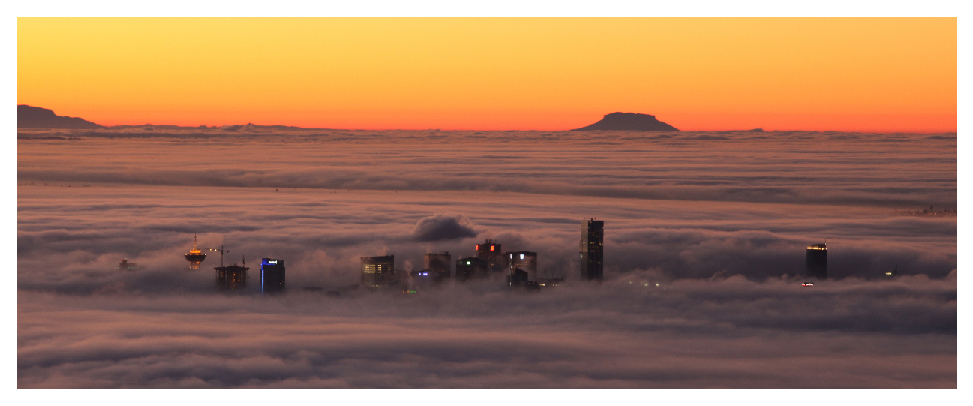
\includegraphics[width=\linewidth]{CypressView}
%  \caption{In the Clouds: Vancouver from Cypress Mountain. Note that the teaser may not be wider than the abstract block.}
%	\label{fig:teaser}
%}

%% Uncomment below to disable the manuscript note
%\renewcommand{\manuscriptnotetxt}{}

%% Copyright space is enabled by default as required by guidelines.
%% It is disabled by the 'review' option or via the following command:
% \nocopyrightspace

\vgtcinsertpkg

%%%%%%%%%%%%%%%%%%%%%%%%%%%%%%%%%%%%%%%%%%%%%%%%%%%%%%%%%%%%%%%%
%%%%%%%%%%%%%%%%%%%%%% START OF THE PAPER %%%%%%%%%%%%%%%%%%%%%%
%%%%%%%%%%%%%%%%%%%%%%%%%%%%%%%%%%%%%%%%%%%%%%%%%%%%%%%%%%%%%%%%%

\begin{document}

%% The ``\maketitle'' command must be the first command after the
%% ``\begin{document}'' command. It prepares and prints the title block.

%% the only exception to this rule is the \firstsection command
\firstsection{Introduction}

\maketitle

Our project involves determining the optimal factors a YouTube video must possess in order to be successful. To quantify success, we will use data from YouTube's trending video list and analyze how these videos have become successful. The Youtube trending list is a front page selection of videos that Youtube has generated using their proprietary algorithm. Youtube has not explained exactly what factors can get a video on the trending list but it is likely some combination of likes, dislikes, comments, views, and category. Videos that end up on the Youtube trending list receive a high level of additional attention and views. Such factors we will look at include: the time of day the video was published, like to dislike ratio, and the most effective video category. We will be looking at YouTube data from five different countries: Canada, Germany, France, the UK and the USA). With the growing influence of the YouTube platform, it is increasingly difficult for videos to garner more attention. This problem is best addressed with a visualization as it makes use of a large amount of data, pulling out the necessary details to display to the user. In this way, anybody would be able to make sense of what the data is communicating with ease. Some potential users of this visualization could simply be any one person with a YouTube account looking to increase the number of views they receive on a video they upload. Users could also include digital marketers and companies trying to increase the success of their promotional campaigns. The general approach we intend to take with this visualization is to present our selected data in a form easily understandable by the user: bar charts, donut charts, and a word cloud. We also intend to help the user to navigate through the data by allowing them to select different factors to display within the visualization.


\subsection{Visualization Tasks}

With the increased use of Youtube as a media platform, more and more content creators are looking to make their mark on the online video landscape. Youtube is not only a platform for creative expression but a marketplace where people make their careers. The goal of our visualization is to provide Youtube content creators with the information they need to make informed decisions that will allow them to maximize the impact of their video. We want to visually illustrate the impact that time of day has on the success of a video and what time of day a content creator should post their content in order to maximize their exposure. To do this we will provide several graphs that show the impact of a video based on the time of day it was posted. Impact can be measured in several different ways. The first is the view count of the video. After view count, statistics such as video count can be used to measure impact. By illustrating these statistics Youtube creators will be able to see the impact their choice of publish time has on video performance. To give creators as much information as possible we will enable them to choose the country or region which they can use to target their specific audience.

In addition to publish time, we want to give creators the opportunity to explore what categories make up the Youtube trending video list as well as what video tags are the most popular. A simple bar chart can measure category popularity while a word cloud made up of the most popular video tags will illustrate what tags are common.

The third task we wish to illustrate is the makeup of how users interact with videos on the trending list. To do this we will compare the average number of likes a video receives with averages dislikes and comments.




\section{Related Work}
Many papers have been written about the problem of visualizing data from social networks. In Slingsby's \textit{“Interactive Tag Maps and Tag Clouds for the Multiscale Exploration of Large Spatio-temporal Datasets”} \cite{4272027},  social media tag maps are discussed.  This approach is another method for visualizing social media data. By creating a tag map of popular YouTube tags, the effects of tags on video's popularity can be visualized. These tag maps would show the most impactful video tags on the YouTube trending video list and allow users to target their video tags more precisely. Similarly, in Viégas' \textit{““Many Eyes: A Site for Visualization at Internet Scale”} \cite{4376131}, approaches for visualization of internet data are discussed. The ManyEyes tool would be another method for visualizing YouTube data.


\section{Methods}

\subsection{Data Source}
The data we will use is the Trending Youtube Video Statistics published by kaggle.com. This data consists of several months of statistics on the top 200 most popular Youtube videos as defined by Youtube in their trending video section. Data sets for several different regions are available including the United States, France, Great Britain, and Canada. 

The data set consists of a flat record. For each video entry, data such as views, likes, dislikes, comment count, and description are provided. The full structure of the data is illustrated in figure \ref{fig:data}.

\subsection{Data Manipulation}
To create this visualization we made use of several different tools. To analyze and organize our data we wrote scripts in Python using the Numpy and Pandas libraries. Pandas allowed us to quickly parse the large csv file with pandas.read\_csv() and then select the columns we needed while Numpy was essential for calculating the data's statistics. The pandas.to\_datetime() function allowed us to quickly parse the timestamp column provided in the data set and with Python's datetime library we were able to convert the column into easily manipulate datetime objects.  Using the numpy.where() and numpy.mean() functions, we could select the columns we needed and calculate the relevant statistics. For example, to select the indices of all videos published between two different times we used np.where(np.logical\_and((timeList $>$ lastHour),  (timeList $<$ nextHour))). To generate a word cloud, we used the tags column of the data and generated a dict that contained all words paired with the count of how many times they appeared in the tags. We took the top 150 of these words for our wordcloud. After analyzing the data plain Python was used to format the output in a form that was readable by our chosen chart creation tool

\subsection{Visualization Construction}

To create the graphs we used the Chart.JS charting library. This library allowed us to easily produce different types of graphs all of which were visually pleasing and interactive. These were integrated into our visualisation webpage using Javascript. The D3 Cloud library was also used to create a word cloud as Chart.JS does not support this feature. The webpage itself with the visualisation settings panel was created with a mixture of HTML, Javascript, and CSS. The jQuery library was used to handle the the user interactions with the site and to respond
accordingly. This includes displaying the appropriate visualisation based on the users? selection. The Materialize framework was utilised so as to provide the site with a well-designed, responsive and modern interface. These were all imported in the HTML head section, allowing them to be used throughout the code.

Bar charts were used to illustrate publish time and categories, a donut chart was used to show the makeup of the video's likes, dislikes, and comment counts, and a word cloud was used to visualize video tags. 

 

\begin{figure}[tb]
 \centering % avoid the use of \begin{center}...\end{center} and use \centering instead (more compact)
 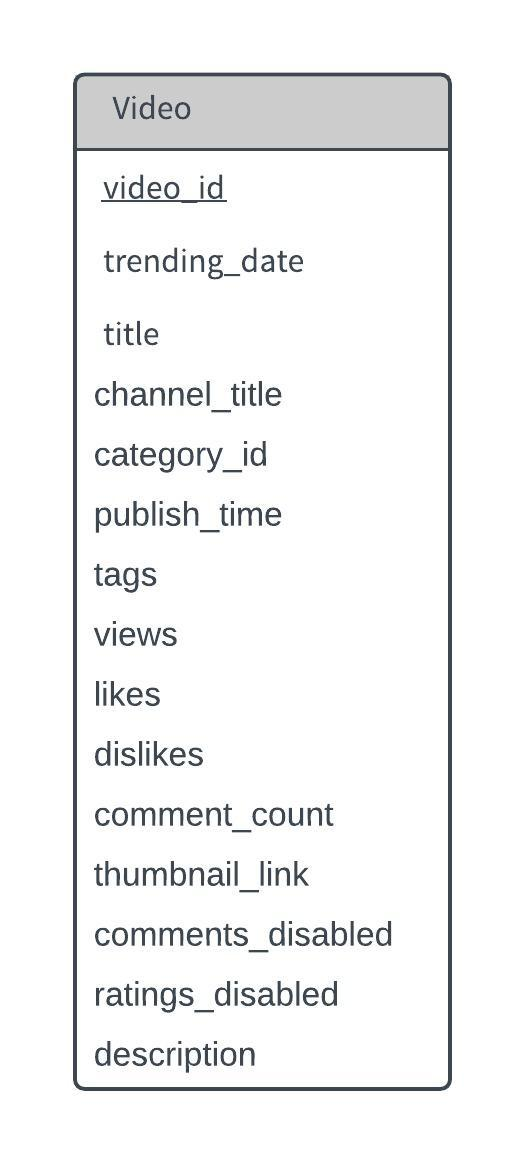
\includegraphics[width=0.6\columnwidth]{erd}
 \caption{A visualization of the Trending YouTube Video Statistics data set}
 \label{fig:data}
\end{figure}


\begin{figure}[tb]
	\centering % avoid the use of \begin{center}...\end{center} and use \centering instead (more compact)
	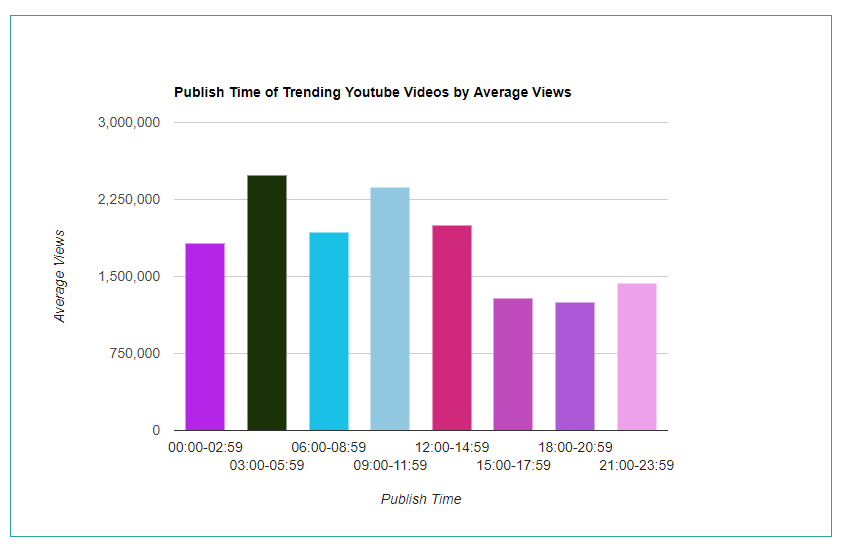
\includegraphics[width=1\columnwidth]{publishtimeviews}
	\caption{A visualization of publish time compared to average view count for the Trending YouTube Video Statistics data set}
	\label{fig:publishtimeviews}
\end{figure}

\section{Results}

The results show a higher view count for videos published between midnight and noon, illustrated in figure \ref{fig:publishtimeviews}. The highest view counts are on videos published between 3:00 AM and 6:00 AM with the lowest being between 6:00 PM and 9:00 PM. Clearly videos published early in the day are more successful. As we can see in figure \ref{fig:publishtimevideocount}, the opposite pattern is observed when looking at the most popular time of day for publishing videos. A strong majority of videos are published within the afternoon and evening hours.

One interesting feature of the data is that the most successful publish time is common to all countries. We expected for different countries to have different top publish times due to differing timezones so this was unexpected. Several possibilities can explain this discrepancy. It is possible that the United States is so impactful in the mediasphere that they choose the most successful publish time even on videos from other countries.  The most successful slot, 3:00 - 6:00 AM PST, is when most of the east coast of the United States is waking up, a common time to access videos and a time accepted by many to be the best time of day to post internet content. We must also wonder if the data we have is labeled accurately. The times are all supposed to be in PST, Youtube's timezone, but looking at the distribution it is possible that the timezones are that of the country where the video was published.

Of the US video categories, music is by far the most popular. Music has the highest views at 5.9 million average views. Of the 16 categories that are featured on the YouTube Trending videos list (not all categories appear), the News and Politics category is by far the least popular with an average view count of 581,000. We see a similar distribution of category views between the different countries with a few exceptions. Science and Technology is far more popular in Great Britain than in the other countries we observed as is News and Politics.

The word cloud presents an interesting view of what tags are popular. Most are unexpected, words such as "the" and "to", but several stand out. "Makeup" is featured quite prominently reflecting the increased popularity of makeup videos on Youtube and we also see words like "iphone", representing the technical review side of the site. 

\begin{figure}[tb]
	\centering % avoid the use of \begin{center}...\end{center} and use \centering instead (more compact)
	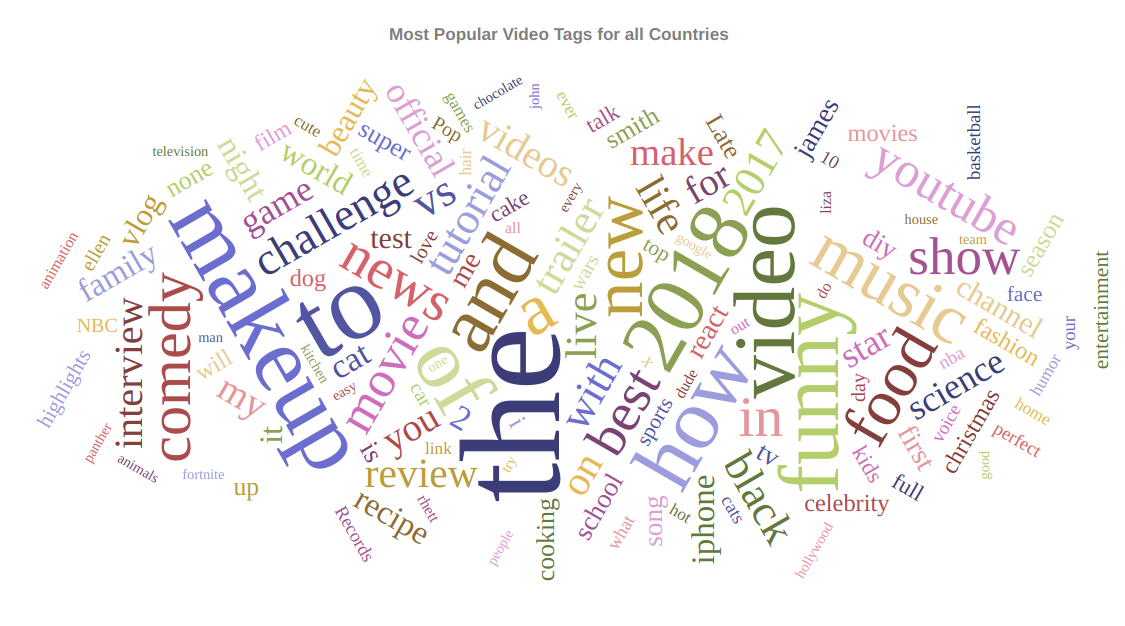
\includegraphics[width=1\columnwidth]{wordcloud}
	\caption{A word cloud of popular tags}
	\label{fig:wordcloud}
\end{figure}


\begin{figure}[tb]
	\centering % avoid the use of \begin{center}...\end{center} and use \centering instead (more compact)
	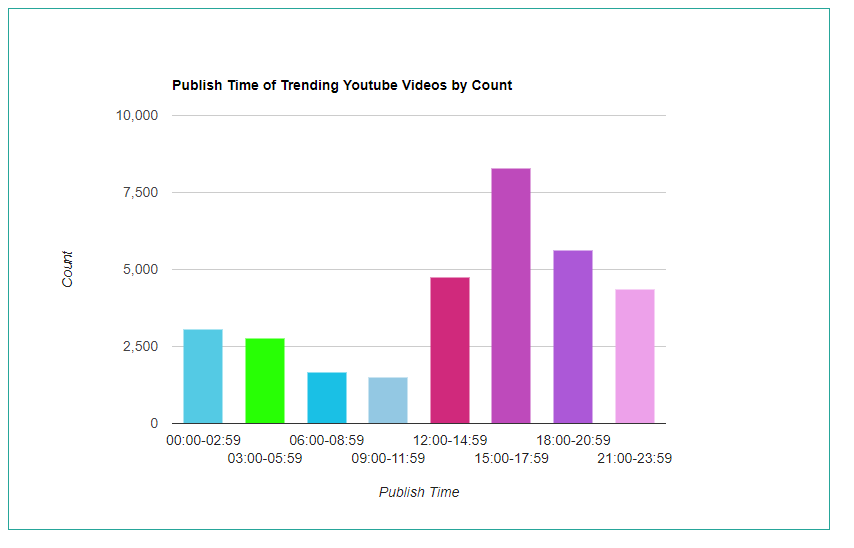
\includegraphics[width=1\columnwidth]{publishtimevideocount}
	\caption{A visualization of publish time compared to number of videos for the Trending YouTube Video Statistics data set}
	\label{fig:publishtimevideocount}
\end{figure}

\begin{figure}[tb]
	\centering % avoid the use of \begin{center}...\end{center} and use \centering instead (more compact)
	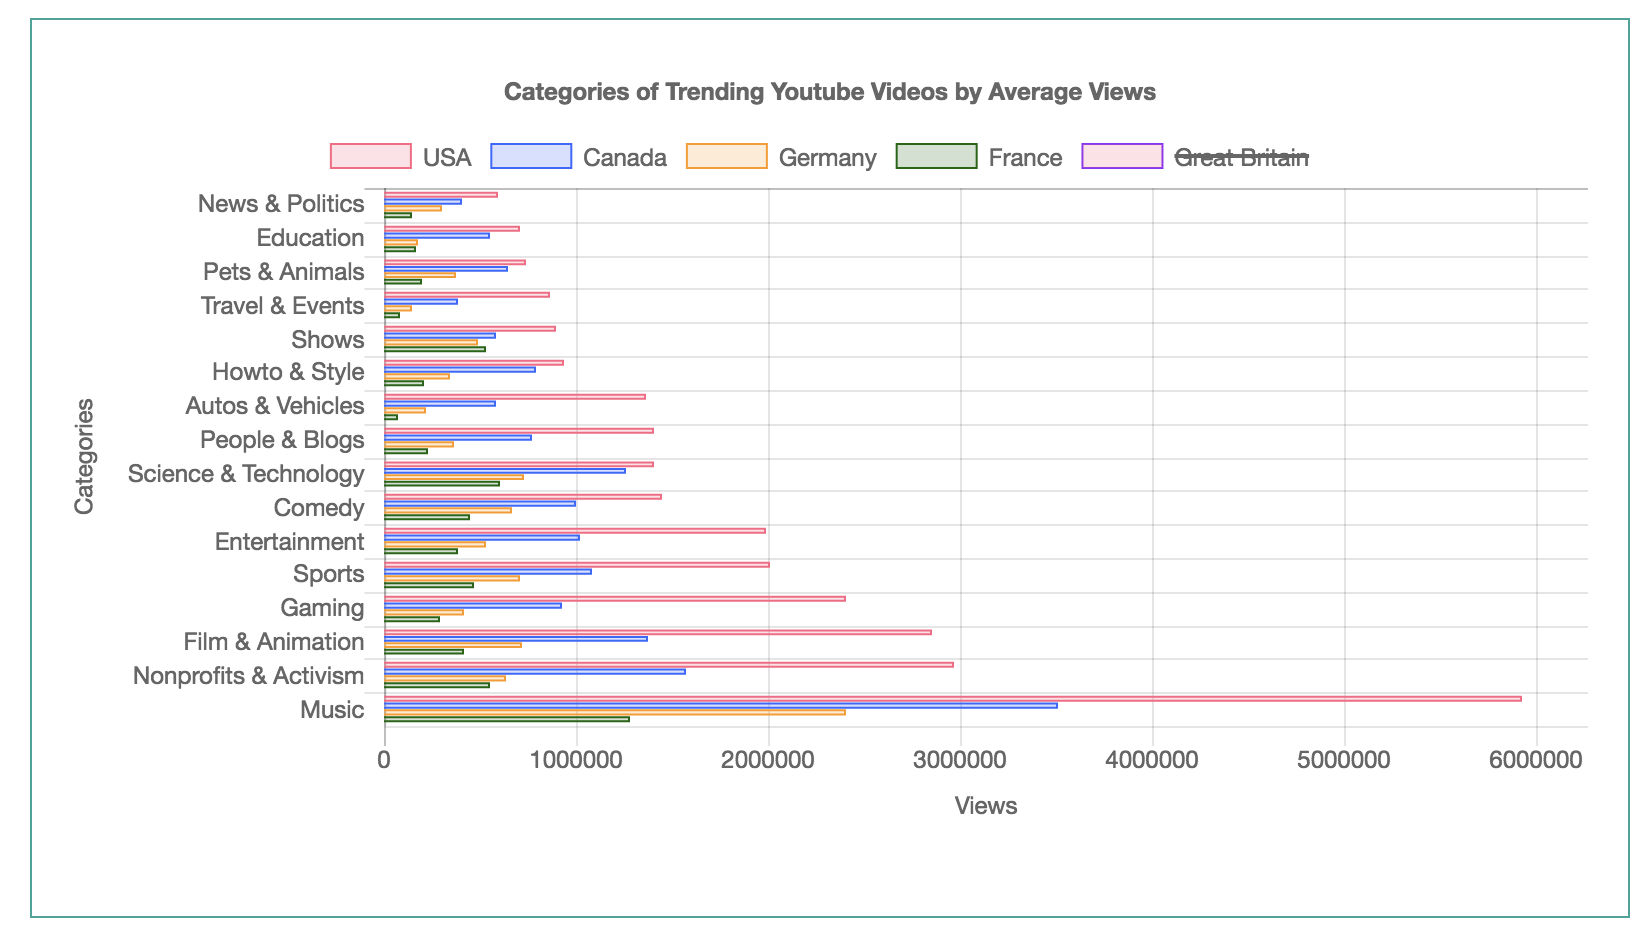
\includegraphics[width=1\columnwidth]{category}
	\caption{A visualization of mean views per video category for the Trending YouTube Video Statistics data set}
	\label{fig:category}
\end{figure}

\section{Contributions}
Michael Giovannoni was responsible for analyzing the data and constructing the necessary data tables for creating the graphs. In addition, he write most of the report and compiled the final submission.

Omar Iltaf was responsible for the visualization applet. He designed the site and wrote all of the html, CSS and most of the javascript.  


\section{Conclusion}

Our visualization allows YouTube content creators to easily see the impact that time of day has on video success and what categories are most popular. Users are able to select the factors that they are interested in and the data is displayed in simple charts. This visualization enables YouTube channel creators to tailor their video publishing to their audience and increase their exposure. 

The most difficult part of this project was dealing with the data. The dataset we were provided was incomplete. In some places values were missing and in others extraneous values were provided, causing the read\_csv function to give us errors. 

If the project were to be continued, it would be helpful to find another dataset, that of non-trending Youtube videos. If we were to compare the two sets we could better visualize exactly what factors get a video to the top of Youtube. As it is, the project shows the makeup of the trending video list but it does not explain exactly which factors are the most influential in the Youtube trending video algorithm. The scope of the algorithm is outside the realm of information visualization but it may be an interesting project for the future. 

This visualization technique may be suitable for other kinds of social network datasets. For example, the same graphs could be used to visualize the most effective times to make a reddit post and the resulting upvotes and downvotes received on those reddit posts. It may also be effective for data from Facebook and a variety of other social networks.  


\bibliographystyle{abbrv-doi}
\bibliography{template}
\end{document}

